% VAE as a network: x -> encoder -> (mu, sigma) -> sampled z -> decoder -> x_hat,
% compared with x by the reconstruction loss, plus a KL term on (mu, sigma).
\documentclass[border=0pt]{standalone}
\usepackage{amsmath,amssymb}
% Shared visual language for the figures of the book.
% Every figure in this directory loads this file so the chapter reads as one system.
% NOTE: no blank lines are allowed inside \tikzset{...} (a blank line emits \par
% and breaks key scanning).
\NeedsTeXFormat{LaTeX2e}
\ProvidesPackage{figstyle}[2026/10/21 Figure style for Free Energy to LLMs]

\RequirePackage{tikz}
\usetikzlibrary{arrows.meta,positioning,calc,fit,shapes.geometric,shapes.misc,%
  backgrounds,matrix,decorations.pathreplacing,decorations.markings,patterns.meta}

% ---------------------------------------------------------------- palette
% Same values as book/preamble/style.tex, prefixed with F.
\definecolor{FNavy}{HTML}{14324A}
\definecolor{FTeal}{HTML}{0E7490}
\definecolor{FSky}{HTML}{E7F5F8}
\definecolor{FOrange}{HTML}{D97706}
\definecolor{FAmber}{HTML}{FFF3D6}
\definecolor{FInk}{HTML}{1F2937}
\definecolor{FSlate}{HTML}{64748B}
\definecolor{FMist}{HTML}{F5F7FA}
\definecolor{FRose}{HTML}{9F1239}
\definecolor{FRoseMist}{HTML}{FFF1F2}

% ---------------------------------------------------------------- semantics
% Teal   = probability / model / data object
% Orange = training objective, cost, or the quantity moved through the system
% Navy   = neutral structure
% Slate  = secondary label or metadata
% Rose   = failure mode, hazard, masked-out region
\tikzset{
  % Lay figures out in millimetres.  A figure designed 168mm wide is included at
  % \textwidth, so its fonts appear at exactly the size written here.
  every picture/.style={x=1mm,y=1mm,font=\small,line cap=round,line join=round},
  % ---- block styles
  nbase/.style={draw,rounded corners=1.2pt,align=center,inner sep=2.4pt,%
    minimum height=7mm,text=FInk},
  nteal/.style={nbase,draw=FTeal,fill=FSky},
  norange/.style={nbase,draw=FOrange,fill=FAmber},
  nnavy/.style={nbase,draw=FNavy,fill=white},
  nsoft/.style={nbase,draw=FSlate!55,fill=FMist},
  nrose/.style={nbase,draw=FRose,fill=FRoseMist},
  ghost/.style={draw=none,fill=none,align=center,inner sep=1pt},
  plain/.style={draw=none,fill=none,align=center,inner sep=0pt},
  % ---- arrows
  ar/.style={-{Latex[length=1.7mm,width=1.35mm]},draw=FSlate,line width=0.75pt},
  ard/.style={ar,dashed},
  arteal/.style={ar,draw=FTeal},
  arorange/.style={ar,draw=FOrange},
  arrose/.style={ar,draw=FRose},
  thickar/.style={ar,line width=1.2pt},
  % ---- text roles
  ftitle/.style={font=\large\bfseries,text=FNavy,align=center},
  ptitle/.style={font=\small\bfseries,text=FNavy,align=center},
  ptitleo/.style={font=\small\bfseries,text=FOrange,align=center},
  lbl/.style={font=\scriptsize,text=FSlate,align=center,inner sep=1pt},
  lblt/.style={lbl,text=FTeal},
  lblo/.style={lbl,text=FOrange},
  lbln/.style={lbl,text=FNavy},
  lblr/.style={lbl,text=FRose},
  sub/.style={font=\scriptsize,text=FSlate!90,align=center,inner sep=1pt},
  monob/.style={font=\ttfamily\scriptsize,text=FInk,inner sep=1pt},
  mathb/.style={font=\small,text=FInk,inner sep=1pt},
  eqn/.style={font=\scriptsize,inner sep=1.5pt,text=FInk},
  % ---- decorations
  brace/.style={decorate,decoration={brace,amplitude=2.4pt},draw=FSlate,%
    line width=0.6pt},
  bracet/.style={brace,draw=FTeal},
  braceo/.style={brace,draw=FOrange},
  axis/.style={draw=FSlate!55,line width=0.6pt},
  guide/.style={draw=FSlate!45,line width=0.5pt,dashed},
  halolabel/.style={font=\scriptsize,text=FInk,fill=white,fill opacity=0.85,%
    text opacity=1,inner sep=1.4pt,align=center},
}

% Figure title above the drawing, anchored at the figure's top-left.
\newcommand{\figtitle}[2][0]{%
  \node[ftitle,anchor=north west,outer sep=0pt] at (#1,0) {#2};}

% Rounded panel behind a subgroup of nodes.
\newcommand{\figpanel}[3][]{%
  \node[draw=FSlate!35,fill=#3,rounded corners=2pt,inner sep=2.6mm,#1] {#2};}

\endinput

% \pix{lower-left x}{lower-left y}{cell size}{filled cells r/c}{blur 0|1}
\newcommand{\pix}[5]{%
  \fill[white] (#1,#2) rectangle ++(6*#3,6*#3);
  \ifnum#5=1
    \begin{scope}
    \clip (#1,#2) rectangle ++(6*#3,6*#3);
    \foreach \r/\c in #4{\fill[FTeal,opacity=0.18] ({#1+(\c-1.5)*#3},{#2+(5.5-\r)*#3}) rectangle ++(2*#3,2*#3);}
    \end{scope}
    \foreach \r/\c in #4{\fill[FTeal!65] ({#1+(\c-1)*#3},{#2+(6-\r)*#3}) rectangle ++(#3,#3);}
  \else
    \foreach \r/\c in #4{\fill[FTeal] ({#1+(\c-1)*#3},{#2+(6-\r)*#3}) rectangle ++(#3,#3);}
  \fi
  \foreach \k in {0,...,6}{%
    \draw[FSlate!30,line width=0.3pt] ({#1+\k*#3},#2) -- ++(0,6*#3);
    \draw[FSlate!30,line width=0.3pt] (#1,{#2+\k*#3}) -- ++(6*#3,0);}
  \draw[FSlate!70,line width=0.5pt] (#1,#2) rectangle ++(6*#3,6*#3);}
% \vecbar{center x}{bottom y}{cells}{fill}
\newcommand{\vecbar}[4]{%
  \foreach \k in {1,...,#3}{\draw[FSlate!70,fill=#4,line width=0.4pt] ({#1-1.4},{#2+(\k-1)*2.4}) rectangle ++(2.8,2.4);}}
\def\seven{1/2,1/3,1/4,1/5,2/5,3/4,4/3,4/4,5/3,6/3}
\def\one{1/3,2/2,2/3,3/3,4/3,5/3,6/2,6/3,6/4}
\begin{document}
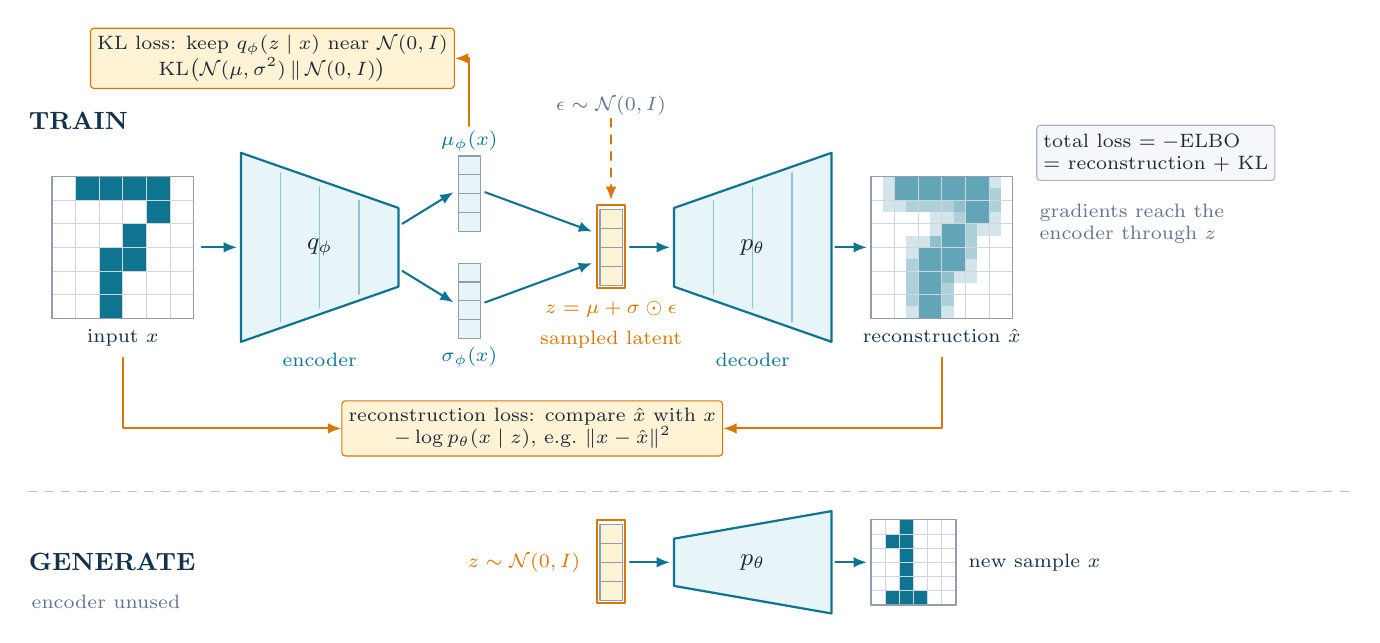
\begin{tikzpicture}
\node[plain,anchor=west,font=\small\bfseries,text=FNavy] at (0,50) {TRAIN};
% ------------------------------------------------------------------ input
\pix{3}{25}{3}{\seven}{0}
\node[lbln,anchor=north] at (12,24) {input $x$};
% ------------------------------------------------------------------ encoder
\fill[FSky,draw=FTeal,line width=0.8pt] (27,22) -- (47,29) -- (47,39) -- (27,46) -- cycle;
\foreach \u in {32,37,42}{\draw[FTeal!45,line width=0.5pt] (\u,{22+7*(\u-27)/20+0.8}) -- (\u,{46-7*(\u-27)/20-0.8});}
\node[mathb] at (37,34) {$q_\phi$};
\node[lblt,anchor=north] at (37,21) {encoder};
\draw[arteal] (22,34) -- (26.5,34);
% ------------------------------------------------------------------ mean and std heads
\vecbar{56}{36}{4}{FSky}
\vecbar{56}{22.4}{4}{FSky}
\node[lblt,anchor=south] at (56,45.8) {$\mu_\phi(x)$};
\node[lblt,anchor=north] at (56,21.8) {$\sigma_\phi(x)$};
\draw[arteal] (47.5,37) -- (54,41);
\draw[arteal] (47.5,31) -- (54,27);
% ------------------------------------------------------------------ sampling
\vecbar{74}{29.2}{4}{FAmber}
\draw[FOrange,line width=0.8pt] (72.2,28.8) rectangle (75.8,39.4);
\node[lblo,anchor=north] at (74,27.6) {$z=\mu+\sigma\odot\epsilon$};
\node[lblo,anchor=north] at (74,23.8) {sampled latent};
\draw[arteal] (58,41) -- (71.6,36);
\draw[arteal] (58,27) -- (71.6,32);
\node[lbl] (eps) at (74,52) {$\epsilon\sim\mathcal N(0,I)$};
\draw[arorange,dashed] (eps.south) -- (74,40);
% ------------------------------------------------------------------ decoder
\fill[FSky,draw=FTeal,line width=0.8pt] (82,29) -- (102,22) -- (102,46) -- (82,39) -- cycle;
\foreach \u in {87,92,97}{\draw[FTeal!45,line width=0.5pt] (\u,{29-7*(\u-82)/20+0.8}) -- (\u,{39+7*(\u-82)/20-0.8});}
\node[mathb] at (92,34) {$p_\theta$};
\node[lblt,anchor=north] at (92,21) {decoder};
\draw[arteal] (76.4,34) -- (81.5,34);
% ------------------------------------------------------------------ reconstruction
\pix{107}{25}{3}{\seven}{1}
\draw[arteal] (102.5,34) -- (106.5,34);
\node[lbln,anchor=north] at (116,24) {reconstruction $\hat x$};
% ------------------------------------------------------------------ losses
\node[norange,font=\scriptsize] (rec) at (64,11) {reconstruction loss: compare $\hat x$ with $x$\\$-\log p_\theta(x\mid z)$, e.g.\ $\|x-\hat x\|^2$};
\draw[arorange] (12,20) |- (rec.west);
\draw[arorange] (116,20) |- (rec.east);
\node[norange,font=\scriptsize] (kl) at (31,58) {KL loss: keep $q_\phi(z\mid x)$ near $\mathcal N(0,I)$\\$\mathrm{KL}\bigl(\mathcal N(\mu,\sigma^2)\,\Vert\,\mathcal N(0,I)\bigr)$};
\draw[arorange] (56,49.4) |- (kl.east);
\node[nsoft,font=\scriptsize,align=left,anchor=west] at (128,46) {total loss $=-\mathrm{ELBO}$\\$=$ reconstruction $+$ KL};
\node[lbl,align=left,anchor=west] at (128,37) {gradients reach the\\encoder through $z$};
\draw[guide] (0,3) -- (168,3);
% ------------------------------------------------------------------ generation
\node[plain,anchor=west,font=\small\bfseries,text=FNavy] at (0,-6) {GENERATE};
\node[lbl,anchor=west] at (0,-11) {encoder unused};
\vecbar{74}{-10.8}{4}{FAmber}
\draw[FOrange,line width=0.8pt] (72.2,-11.2) rectangle (75.8,-0.6);
\node[lblo,anchor=east] at (70.5,-6) {$z\sim\mathcal N(0,I)$};
\fill[FSky,draw=FTeal,line width=0.8pt] (82,-9) -- (102,-12.5) -- (102,0.5) -- (82,-3) -- cycle;
\node[mathb] at (92,-6) {$p_\theta$};
\draw[arteal] (76.4,-6) -- (81.5,-6);
\pix{107}{-11.4}{1.8}{\one}{0}
\draw[arteal] (102.5,-6) -- (106.5,-6);
\node[lbln,anchor=west] at (119,-6) {new sample $x$};
\end{tikzpicture}
\end{document}
